%-----------------------------------------------------------------------------%
%	Packages & Other Configurations
%-----------------------------------------------------------------------------%
\RequirePackage{fix-cm}  % Fix Font shape `OT1/cmr/m/n' size substitution.
\documentclass[a4paper,10pt]{article}
\usepackage[top=0.5in, bottom=0.6in, left=1in, right=0.9in]{geometry}
\usepackage[utf8]{inputenc} %add acents
\usepackage{setspace} % command \doublespacing etc...
\usepackage{lineno} % number lines
\usepackage{epsf,epsfig} % includegraphics [pdf, png etc]
\usepackage{amsmath} %adicionei esse pacote pra vc poder usar o draft%
\usepackage{textcomp} %símbolos de texto
\usepackage{natbib} % bibtex - adicionar referencia
% \usepackage{url} % for bibtex - configuracoes de urls
\usepackage{tabularx} % for tables
\usepackage[hidelinks]{hyperref}  % Add URL links.
% \usepackage[bookmarks=false,colorlinks=true,urlcolor={green},linkcolor={green},pdfstartview={XYZ null null 1.22}]{hyperref} %all references

%-----------------------------------------------------------------------------%
%	Adicionar a Watermark
%-----------------------------------------------------------------------------%
\usepackage{draftwatermark}
\SetWatermarkAngle{45}
\SetWatermarkLightness{0.9}
\SetWatermarkFontSize{5cm}
\SetWatermarkScale{0.3}
\SetWatermarkText{Exercícios 2 - Oceanografia}

%-----------------------------------------------------------------------------%
%	Informações sobre o PDF
%-----------------------------------------------------------------------------%

\pdfinfo{%
  /Title    (GEO232 - Exercícios 2)
  /Author   (Ju Leonel)
  /Creator  (Ju Leonel)
  /Producer (Ju Leonel)
  /Subject  (Intro oceanografias)
  /Keywords (Intro oceanografia, Exercícios 2)}

%-----------------------------------------------------------------------------%
%	Documento
%-----------------------------------------------------------------------------%
\title{GEO232 - Introdução à Oceanografia - IGEO-UFBA - Exercícios 2}
\author{\vspace{-10ex}}
\date{\vspace{-10ex}}

\begin{document}

  \maketitle
  %\doublespacing
  \onehalfspace

  \begin{tabular*} {0.9\textwidth}{@{\extracolsep{\fill} } l l}
    \hline
    Professora: Juliana Leonel & Atendimento: Sextas-feiras \\
    E-mail: \href{mailto:jleonel@ufba.br}{jleonel@ufba.br} & Horário atendimento: 13:00-14:00 \\
    Aulas: Terças e Quintas-Feiras & Local atendimento: IGEO - Sala 10 - 2\textsuperscript{o} andar\\
    Horário- Aulas: 10:40 - 12:30 & Homepage: \url{http://juoceano.github.io/introductiontooceanography}\\
    \hline
  \end{tabular*}

  \vspace{3ex}

    \section{Exercício de Salinidade}

    \noindent

    A figura abaixo representa a distribuição de salinidade na superfície dos oceanos. Observe atentamente  a figura e descreva como ocorre a distribuição horizontal de salinidade nos oceanos. Justifique a sua resposta.

\begin{figure}[h!]
  \centering
    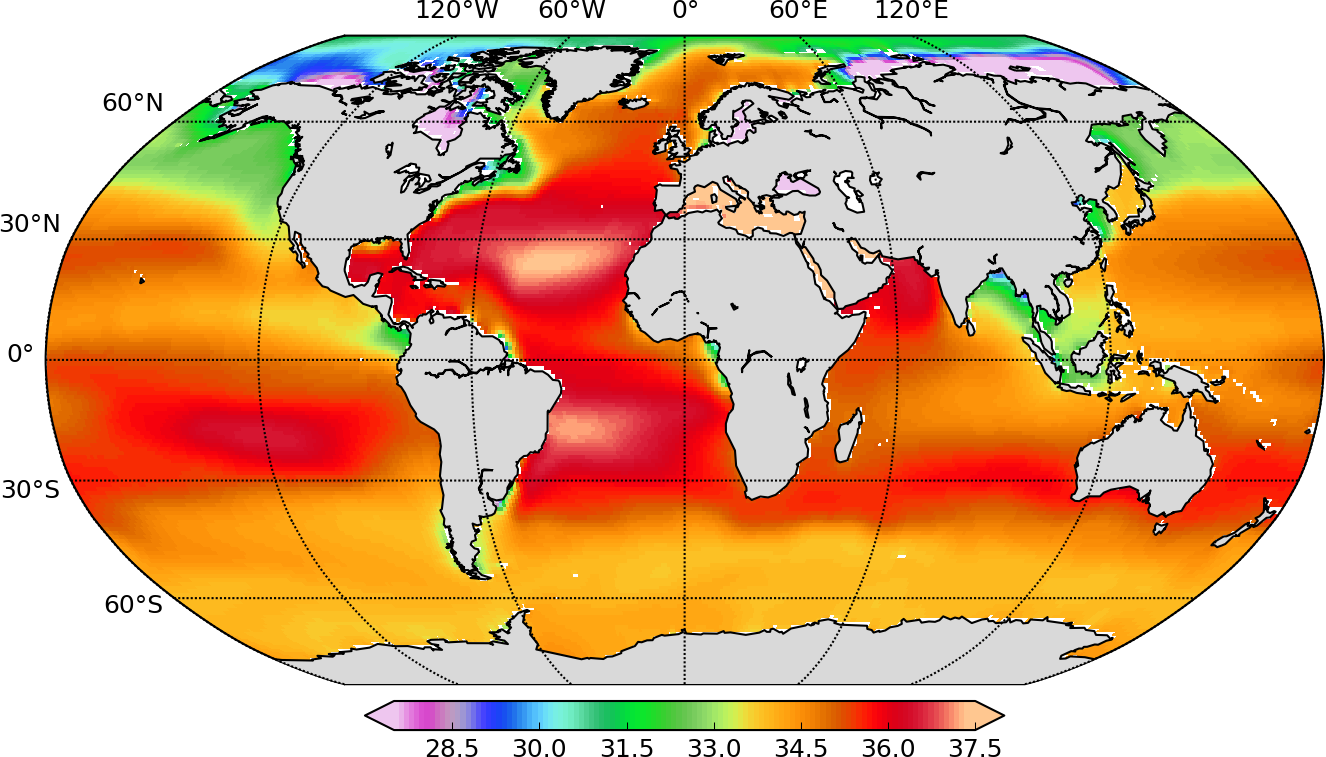
\includegraphics[width=0.95\textwidth]{surface_salinity_woa09}
  \caption{Distribuição de salinidade em g kg$^{-1}$}
\end{figure}


%\clearpage %termina o texto e tudo que estiver flutuante se encaixa ali
%\newpage % começa uma nova página
%\bibliographystyle{chicago} % estilo que vai sair a bibliografia (posso usar outros)
%\bibliography{references_ju} %entre chaves vai o nome do arquivo de referencias

\end{document}
